\documentclass{beamer}
\usepackage{graphicx}
\usepackage{amsmath, amsthm, amsfonts, amssymb, mathrsfs, mathtools, caption, subcaption}
\usepackage{textcomp} % straigth apos
\usepackage{tikz}
\usepackage{verbatim}
\usepackage{tikzit}
\usepackage{listings}
\usepackage[ruled,vlined, linesnumbered]{algorithm2e}
\usepackage{algorithmic,float}
\usepackage[
  % audience=short
  audience=long
]{beameraudience}

\usetikzlibrary {arrows.meta,automata,positioning} 
\usetikzlibrary{automata}

\usefonttheme{serif}

\theoremstyle{definition}

\setbeamercovered{invisible}

\setbeamertemplate{theorems}[numbered]
\setbeamertemplate{lemma}[numbered]
\newtheorem{remark}{Remark}

\usetheme{Madrid}
\useoutertheme{tree} % Alternatively: miniframes, infolines, split
\useinnertheme{circles}


\setbeamertemplate{headline}
{%
  \leavevmode%
  \begin{beamercolorbox}[wd=.5\paperwidth,ht=2.5ex,dp=1.125ex]{section in head/foot}%
    \hbox to .5\paperwidth{\hfil\insertsectionhead\hfil}
  \end{beamercolorbox}%
  \begin{beamercolorbox}[wd=.5\paperwidth,ht=2.5ex,dp=1.125ex]{subsection in head/foot}%
    \hbox to .5\paperwidth{\hfil\insertsubsectionhead\hfil}
  \end{beamercolorbox}%
}

\setbeamertemplate{section in toc}{%
  \inserttocsectionnumber.~\inserttocsection}
\setbeamercolor{section in toc}{fg=black}
\setbeamercolor{subsection in toc}{fg=structure}
\setbeamertemplate{subsection in toc}{%
  \hspace{1.2em}{\tiny\inserttocsectionnumber.\inserttocsubsectionnumber}~\small\inserttocsubsection\par}

\setbeamertemplate{footline}{} % Remove footer
\setbeamertemplate{navigation symbols}{} % Remove navigation symbols


% \setbeamertemplate{bibliography item}{\insertbiblabel.~\insertbibitem}

\definecolor{maincolor}{RGB}{78, 145, 94}

\usecolortheme[named=maincolor]{structure}

\title[End-of-studies internship]{Verification in Isabelle/HOL of Hopcroft’s algorithm for minimizing DFAs including runtime analysis}
\author[V. Trélat]{
    Vincent Trélat\\
    \small{supervised by Prof. Dr. Tobias Nipkow and Dr. Peter Lammich}
}
\institute[TUM]{Technical University of Munich\\Chair for Logic and Verification}
\date{September 2023}

\newcommand{\prompt}[1]{vtrelat@home:\raisebox{0.5ex}{\texttildelow}\$ #1}

% Outline:
% - Life in Munich
% - TUM and the Chair for Logic and Verification
%     - Teaching
%     - Research : Isabelle
% - Introduce the internship
%     - The algorithm
%     - Verification of correctness
%     - Verification of time complexity


\begin{document}

\begin{frame}
\begin{figure}
\centering
\hfill

\includegraphics[height=9mm]{../img/logoartem.png}\hfill

\includegraphics[height=9mm]{../img/logoTUM.png}\hfill

\includegraphics[height=9mm]{../img/logoisabelle.png}\hfill
\hfill
\end{figure}
\titlepage
\end{frame}

\begin{frame}
    \frametitle{Outline}
    \tableofcontents
\end{frame}

\section{Living in Munich}
\subsection{The city}

\begin{frame}
    \only<1>{
    \begin{figure}
        \centering
        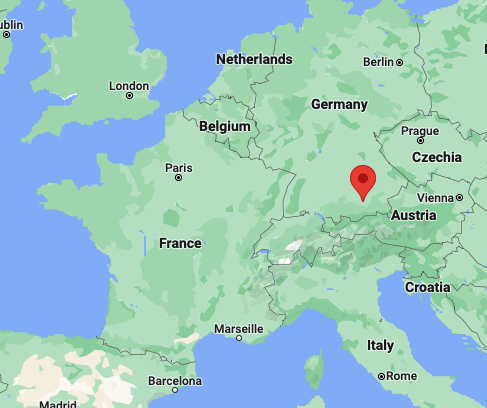
\includegraphics[width=0.7\textwidth]{img/map.png}
        \caption{Location of Munich}
    \end{figure}
    }
    \only<2>{
    \begin{figure}
        \centering
        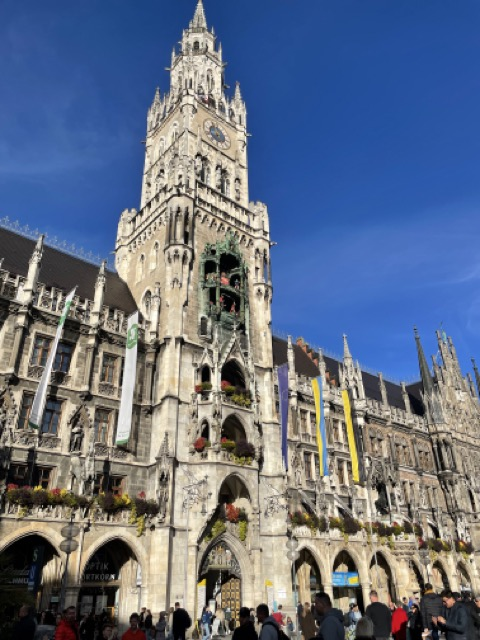
\includegraphics[height=4cm]{img/munich1.jpeg}
        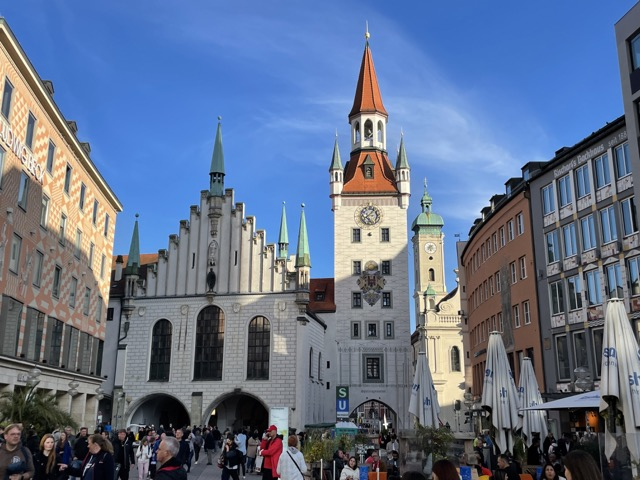
\includegraphics[height=4cm]{img/munich2.jpeg}
        \vfill
        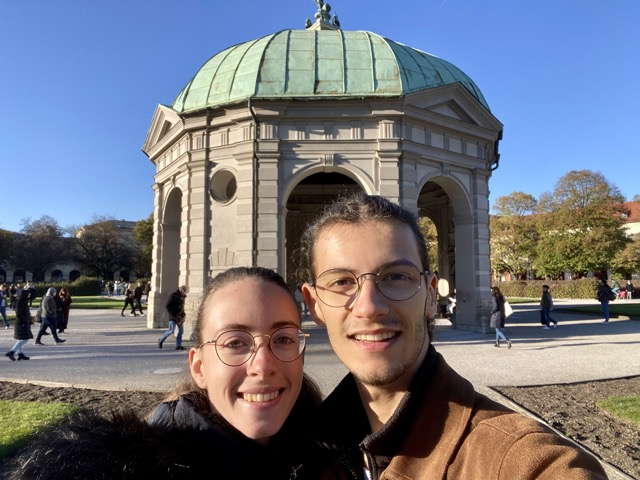
\includegraphics[height=4cm]{img/munich3.jpeg}
        \caption{Some photos of Munich}
    \end{figure}
    }
    \onslide<3->{
    \begin{figure}
        \centering
        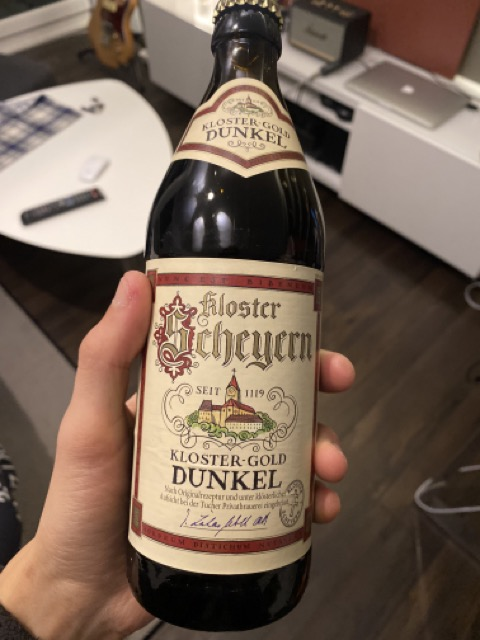
\includegraphics[height=3cm]{img/beer0.jpeg}
        \onslide<4->{
\includegraphics[height=3.2cm]{img/beer1.jpeg}}
        \onslide<5->{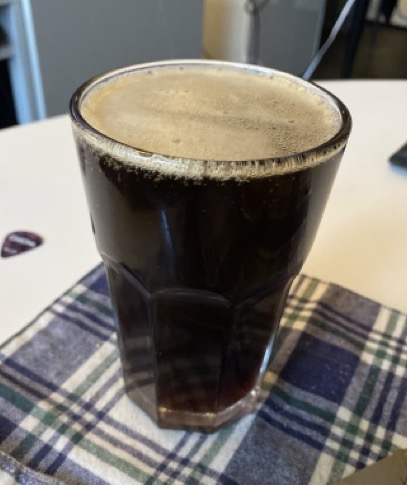
\includegraphics[height=3.2cm]{img/beer2.jpeg}}
        \onslide<6->{
\includegraphics[height=3.2cm]{img/beer3.jpeg}}\\
        \vfill
        \onslide<7->{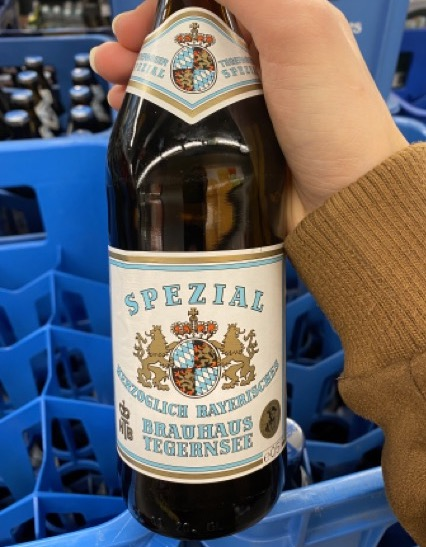
\includegraphics[height=3.2cm]{img/beer4.jpeg}}
        \onslide<8->{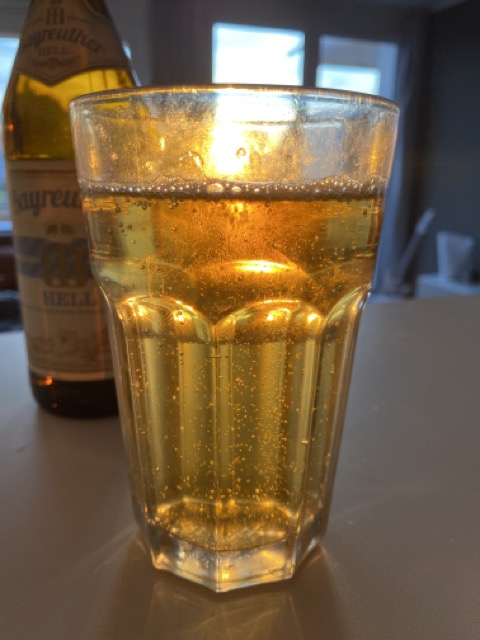
\includegraphics[height=3.2cm]{img/beer5.jpeg}}
        \onslide<9->{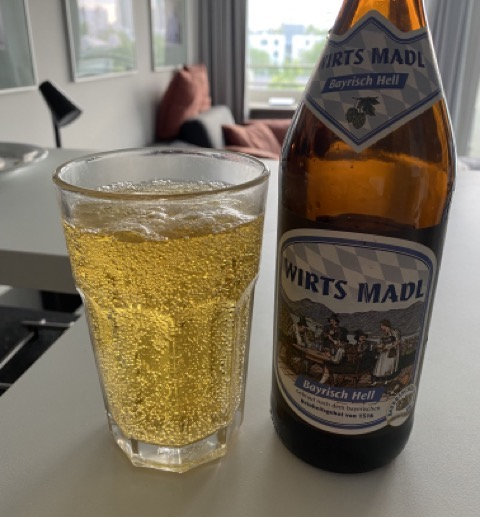
\includegraphics[height=3.2cm]{img/beer6.jpeg}}
        \onslide<10->{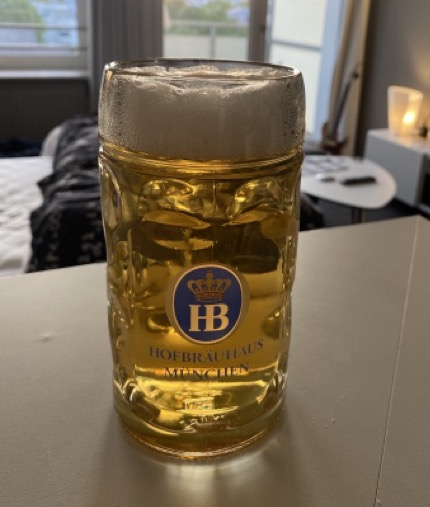
\includegraphics[height=3.2cm]{img/beer7.jpeg}}
    \end{figure}
    }
\end{frame}

\subsection{Technical University of Munich}

\begin{frame}
    \begin{figure}
        \begin{subfigure}{0.3\textwidth}
            \centering
            
\includegraphics[height=1cm]{../img/logoTUM.png}\\
            \vspace*{1cm}
            
\includegraphics[height=1.5cm]{../img/logoisabelle.png}
        \end{subfigure}
        \begin{subfigure}{0.69\textwidth}
            \centering
            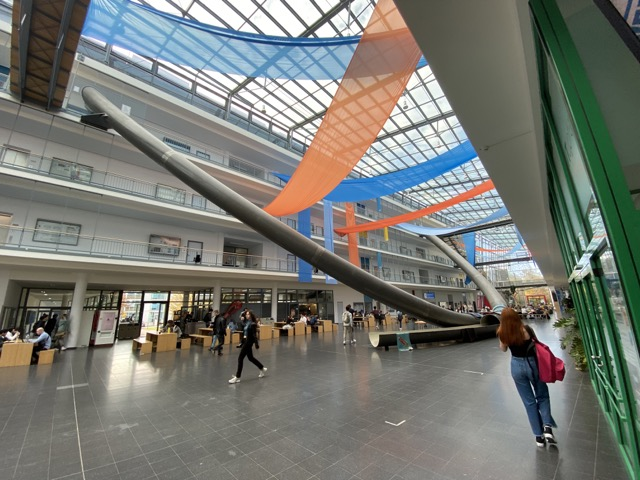
\includegraphics[height=6cm]{img/TUM.jpeg}
        \end{subfigure}
        \caption{Technical University of Munich (TUM)}
    \end{figure}
\end{frame}

\section{Hopcroft's algorithm}

\begin{frame}
    \tableofcontents[currentsection]
\end{frame}

\subsection{DFA minimization by example}
\begin{frame}
    \centering
    \begin{tikzpicture}[shorten >=1pt,node distance=3cm, on grid, >={Stealth[round]},initial text=,
        every state/.style={draw=maincolor,very thick,fill=maincolor!20}]
     
        \node[state, initial] (q0) {$q_0$};
        \node[state, above of=q0] (q1) {$q_1$};
        \node[state, accepting, right of=q0] (q2) {$q_2$};
        \node[state, accepting, above of=q2] (q3) {$q_3$};
        \node[state, accepting, right of=q2] (q4) {$q_4$};
        \node[state, right of=q3] (q5) {$q_5$};

        \path[->] (q0) edge[bend left] node[left]{$0$} (q1);
        \path[->] (q0) edge node[below]{$1$} (q2);
        \path[->] (q1) edge[bend left] node[right]{$0$} (q0);
        \path[->] (q1) edge node[above]{$1$} (q3);
        \path[->] (q2) edge node[below]{$0$} (q4);
        \path[->] (q2) edge node[left=.3cm]{$1$} (q5);
        \path[->] (q3) edge node[above]{$1$} (q5);
        \path[->] (q3) edge node[above=.3cm]{$0$} (q4);
        \path[->] (q4) edge[loop right] node[right]{$0$} (q4);
        \path[->] (q4) edge node[right]{$1$} (q5);
        \path[->] (q5) edge[loop right] node[right]{$0,1$} (q5);
    \end{tikzpicture}
\end{frame}

\begin{frame}
    \centering
    \begin{tikzpicture}[shorten >=1pt,node distance=3cm, on grid, >={Stealth[round]},initial text=,
        every state/.style={draw=maincolor,very thick,fill=maincolor!20}]
     
        \node[state, initial] (Q0) {$q_0, q_1$};
        \node[state, accepting, right of=Q0] (Q1) {$q_2,q_3,q_4$};
        \node[state, right of=Q1] (Q2) {$q_5$};

        \path[->] (Q0) edge[loop above] node[above]{$0$} (Q0);
        \path[->] (Q0) edge node[above]{$1$} (Q1);
        \path[->] (Q1) edge[loop above] node[above]{$0$} (Q1);
        \path[->] (Q1) edge node[above]{$1$} (Q2);
        \path[->] (Q2) edge[loop above] node[above]{$0,1$} (Q2);
    \end{tikzpicture}
\end{frame}

\subsection{Towards a formal definition...}

\begin{frame}
    Formalization
\end{frame}

\end{document}